\section{UI-Bibliotheken und Komponenten}

\begin{definition}{Overview}
\begin{itemize}
  \item Frameworks und Bibliotheken
  \item DOM-Scripting und Abstraktionen
  \item JSX und SJDON
  \item Eigene Bibliothek: SuiWeb
\end{itemize}
\end{definition}

\subsection{Frameworks und Bibliotheken}

\begin{definition}{Framework vs. Bibliothek}
    \begin{itemize}
        \item \textbf{Bibliothek}: 
            \begin{itemize}
                \item Kontrolle beim eigenen Programm
                \item Funktionen werden nach Bedarf verwendet
                \item Beispiel: jQuery
            \end{itemize}
            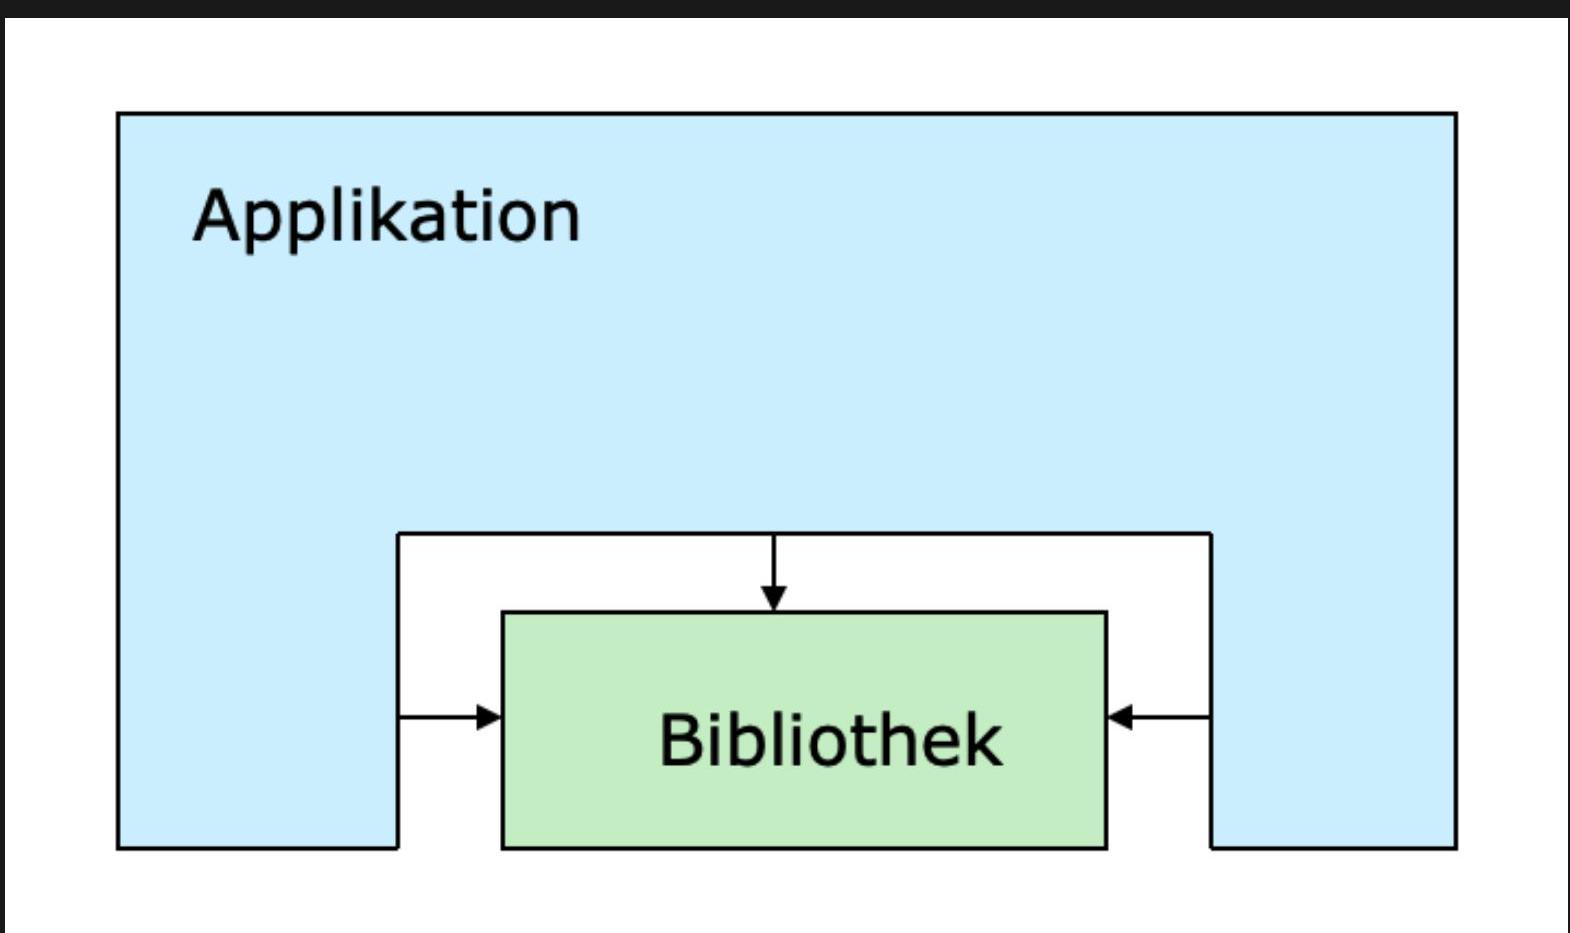
\includegraphics[width=0.5\linewidth]{images/2025_01_02_22162ee5453ad0230328g-04}
        \item \textbf{Framework}: 
            \begin{itemize}
                \item Rahmen für die Anwendung
                \item Kontrolle liegt beim Framework
                \item "Hollywood-Prinzip": don't call us, we'll call you
            \end{itemize}
            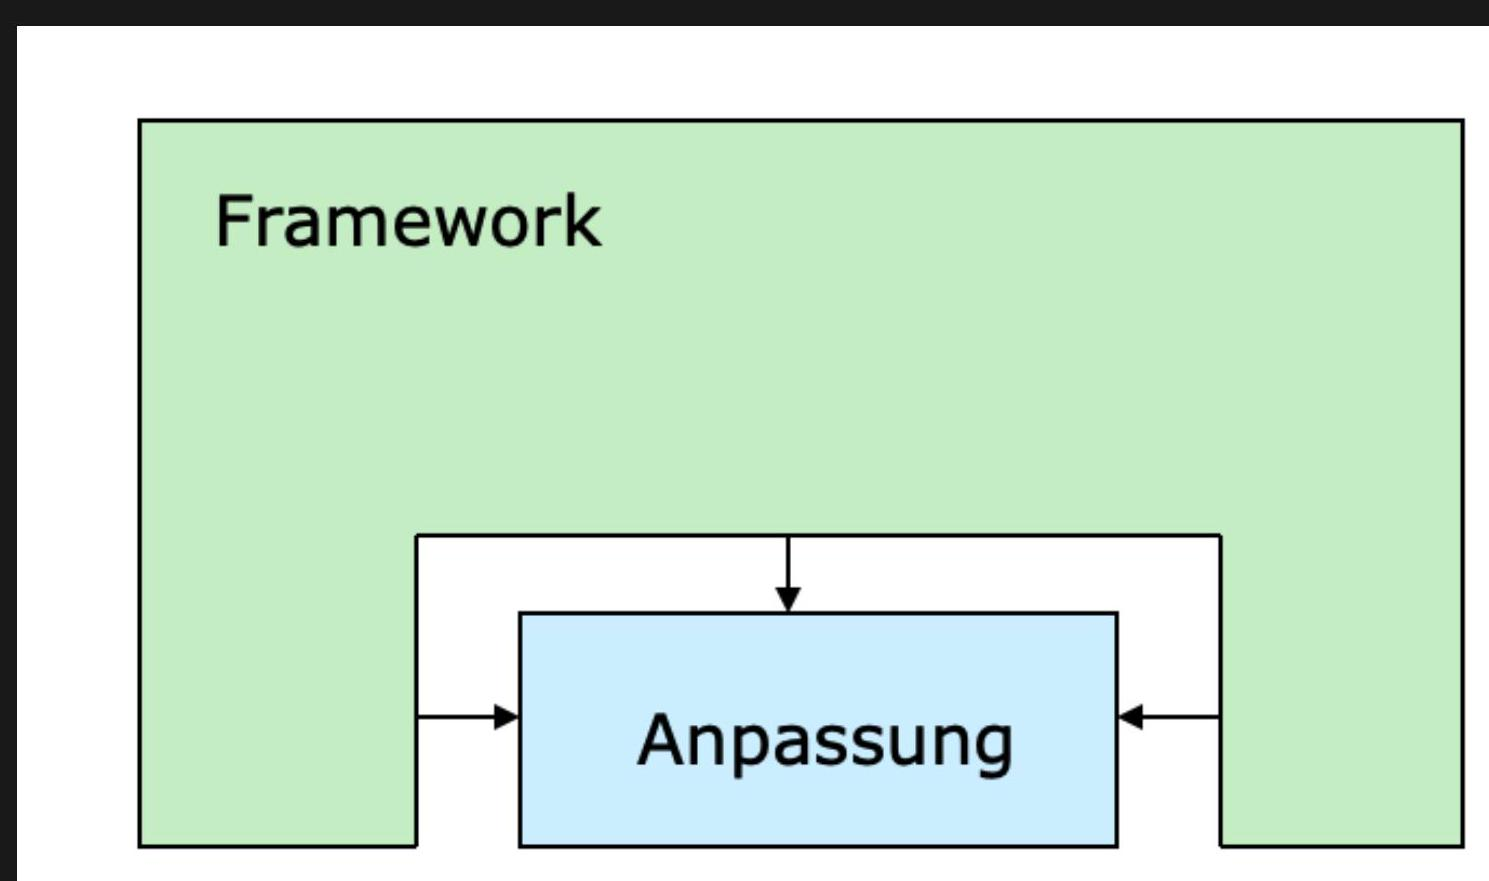
\includegraphics[width=0.5\linewidth]{images/2025_01_02_22162ee5453ad0230328g-05}
    \end{itemize}
\end{definition}

\begin{definition}{ANSÄTZE IM LAUF DER ZEIT}
\begin{itemize}
  \item Statische Webseiten
  \item Inhalte dynamisch generiert (CGI z.B. Shell Scripts, Perl)
  \item Serverseitig eingebettete Scriptsprachen (PHP)
  \item Client Scripting oder Applets (JavaScript, Java Applets, Flash)
  \item Enterprise Application Server (Java, Java EE)
  \item MVC Server-Applikationen (Rails, Django)
  \item JavaScript Server (Node.js)
  \item Single Page Applikationen (SPAs)
\end{itemize}
\end{definition}

\begin{definition}{SERVERSEITE}
\begin{itemize}
  \item Verschiedene Technologien möglich
  \item Zahlreiche Bibliotheken und Frameworks
  \item Verschiedene Architekturmuster
  \item Häufig: Model-View-Controller (MVC)
  \item Beispiel: Ruby on Rails
\end{itemize}
\end{definition}

\begin{concept}{Architektur}
\begin{itemize}
    \item \textbf{MVC (Model-View-Controller)}:
        \begin{itemize}
            \item Model: Repräsentiert Daten und Geschäftslogik, können Observer über Zustandsänderungen informieren
            \item View: Bildet UI (z.B. HTML/CSS), kommuniziert mit Controller
            \item Controller: Verarbeitet Eingaben (z.B. Clicks), aktualisiert Model
        \end{itemize}
    \item \textbf{Single Page Apps (SPAs)}:
        \begin{itemize}
            \item Vermeidet Neuladen von Seiten
            \item Inhalte dynamisch nachgeladen (Ajax, REST)
            \item Bessere Usability durch schnellere UI-Reaktion
        \end{itemize}
\end{itemize}
\end{concept}

\begin{concept}{Model-View-Controller (MVC)}
    \begin{itemize}
        \item \textbf{Models}
            \begin{itemize}
                \item Repräsentieren anwendungsspezifisches Wissen und Daten
                \item Ähnlich Klassen: User, Photo, Todo, Note
            \end{itemize}
        \item \textbf{Views}
            \begin{itemize}
                \item Bilden die Benutzerschnittstelle
                \item Meist HTML/CSS basiert
            \end{itemize}
        \item \textbf{Controllers}
            \begin{itemize}
                \item Verarbeiten Eingaben
                \item Aktualisieren Models
                \item Steuern View-Aktualisierung
            \end{itemize}
    \end{itemize}
\end{concept}

\begin{definition}{RUBY ON RAILS}
\begin{itemize}
  \item Serverseitiges Framework, basierend auf MVC
  \item Programmiersprache: Ruby\\
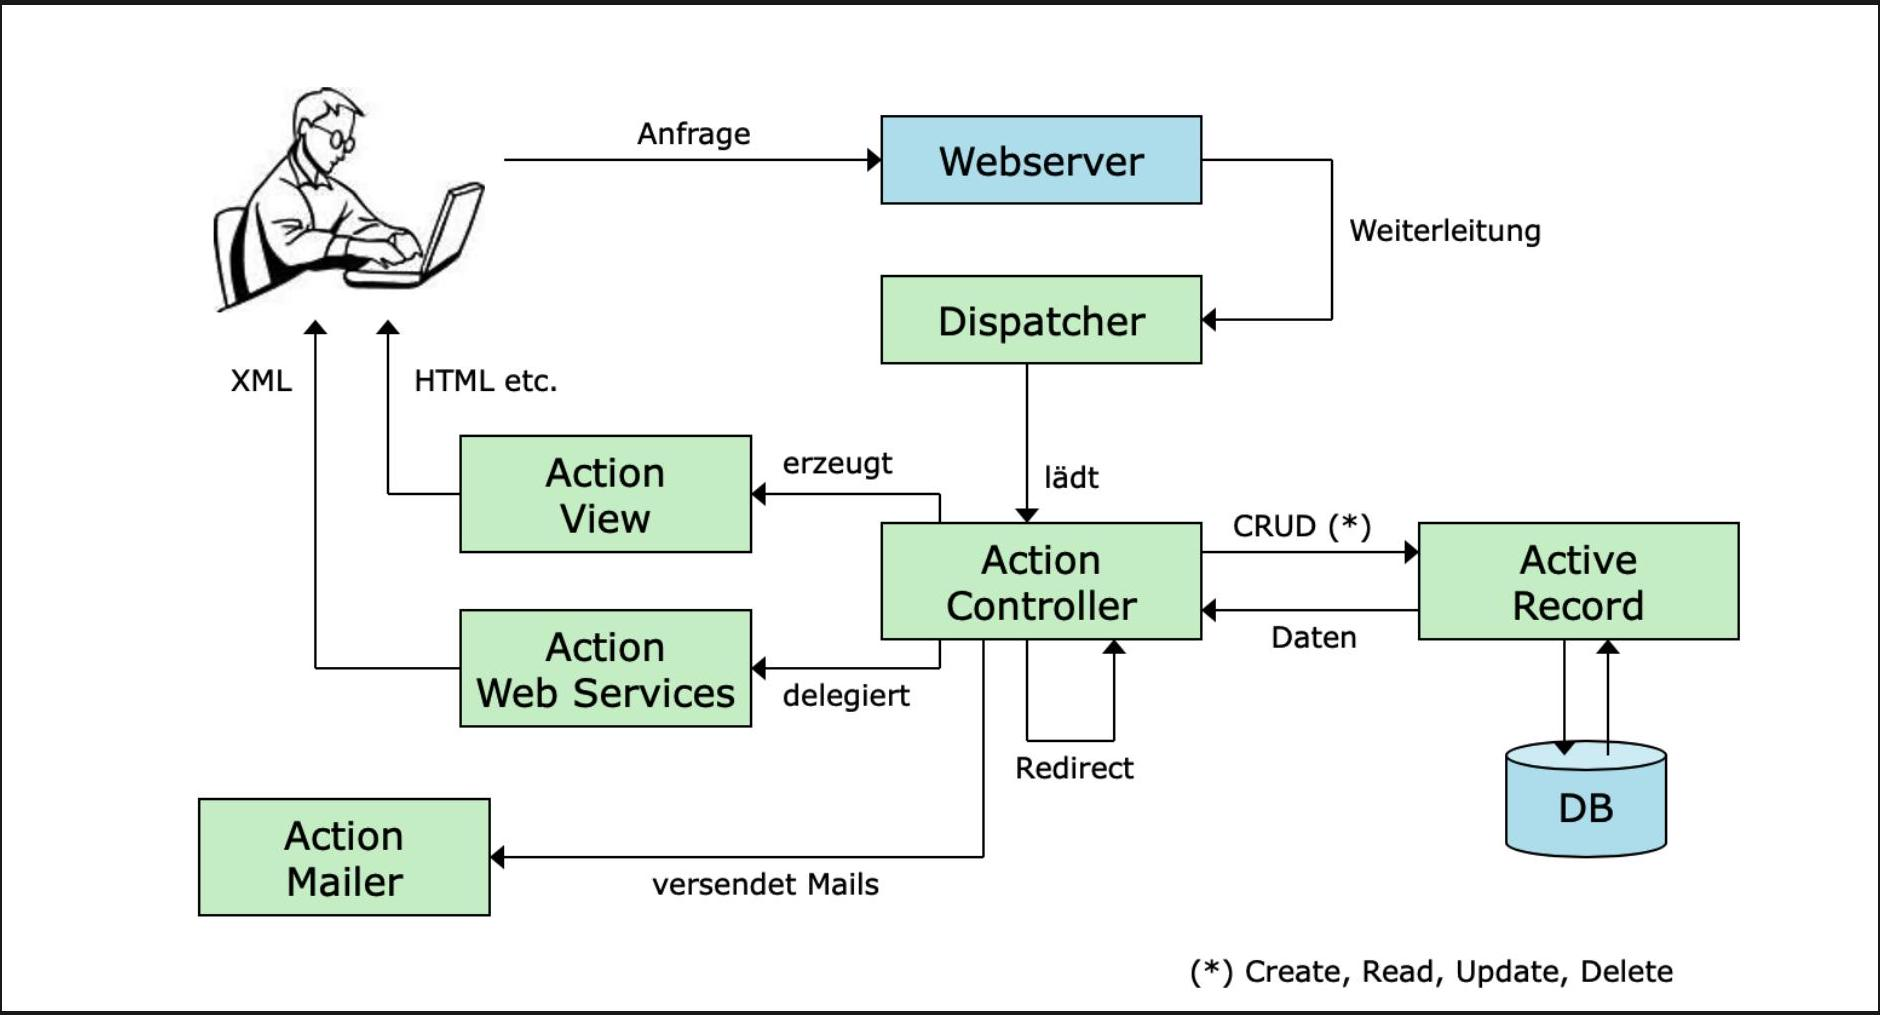
\includegraphics[width=\linewidth]{images/2025_01_02_22162ee5453ad0230328g-09}
\end{itemize}
\end{definition}

\begin{definition}{FOKUS AUF DIE CLIENT-SEITE}
\begin{itemize}
  \item Programmlogik Richtung Client verschoben
  \item Zunehmend komplexe User Interfaces
  \item Asynchrone Serveranfragen, z.B. mit Fetch
  \item Gute Architektur der Client-App wesentlich
  \item Diverse Frameworks und Bibliotheken zu diesem Zweck
\end{itemize}
\end{definition}

\begin{concept}{Komponentenbasierte Entwicklung}
    Grundprinzipien:
    \begin{itemize}
        \item UI in wiederverwendbare Komponenten aufteilen
        \item Klarer Datenfluss (Props down, Events up)
        \item Deklarativer Ansatz
        \item Komponenten können verschachtelt werden
        \item Zustandsverwaltung in Komponenten
        \item Container vs. Präsentations-Komponenten
    \end{itemize}
\end{concept}

\pagebreak

\subsection{DOM-Scripting und Abstraktionen}

\begin{definition}{DOM-SCRIPTING}
\begin{itemize}
  \item Zahlreiche Funktionen und Attribute verfügbar
  \item Programme werden schnell unübersichtlich
  \item Gesucht: geeignete Abstraktionen
\end{itemize}
\end{definition}

\begin{definition}{AUFGABE}
\begin{itemize}
  \item Zum Vergleich der verschiedenen Ansätze
  \item Liste aus einem Array erzeugen
\end{itemize}
\end{definition}

\begin{verbatim}
/* gegeben: */
let data = ["Maria", "Hans", "Eva", "Peter"]
<!-- DOM-Struktur entsprechend folgendem Markup aufzubauen: -->
<ul>
    <li>Maria</li>
    <li>Hans</li>
    <li>Eva</li>
    <li>Peter</li>
</ul>
\end{verbatim}

\begin{definition}{DOM-SCRIPTING}
\begin{verbatim}
function List (data) {
    let node = document.createElement("ul")
    for (let item of data) {
        let elem = document.createElement("li")
        let elemText = document.createTextNode(item)
        elem.appendChild(elemText)
        node.appendChild(elem)
    }
    return node
}
\end{verbatim}
\end{definition}

\begin{itemize}
  \item Erste Abstraktion: Listen-Komponente
  \item Basierend auf DOM-Funktionen
\end{itemize}

\begin{definition}{DOM-SCRIPTING}
\begin{verbatim}
function init () {
    let app = document.querySelector(".app")
    let data = ["Maria", "Hans", "Eva", "Peter"]
    render(List(data), app)
}
function render (tree, elem) {
    while (elem.firstChild) { elem.removeChild(elem.firstChild) }
    elem.appendChild(tree)
}
\end{verbatim}
\end{definition}

\begin{definition}{DOM-SCRIPTING VERBESSERT}
\begin{verbatim}
function elt (type, attrs, ...children) {
    let node = document.createElement(type)
    Object.keys(attrs).forEach(key => {
        node.setAttribute(key, attrs[key])
    })
    for (let child of children) {
        if (typeof child != "string") node.appendChild(child)
        else node.appendChild(document.createTextNode(child))
    }
    return node
}
\end{verbatim}
\end{definition}

\begin{definition}{DOM-SCRIPTING VERBESSERT}
\begin{itemize}
  \item Damit vereinfachte List-Komponente möglich
  \item DOM-Funktionen in einer Funktion elt gekappselt
\end{itemize}

\begin{verbatim}
function List (data) {
    return elt("ul", {}, ...data.map(item => elt("li", {}, item)))
}
\end{verbatim}
\end{definition}


\subsubsection{JQUERY}

\begin{verbatim}
function List (data) {
    return $("<ul>").append(...data.map(item => $("<li>").text(item)))
}
function render (tree, elem) {
    while (elem.firstChild) { elem.removeChild(elem.firstChild) }
    $(elem).append(tree)
}
\end{verbatim}

\begin{itemize}
  \item List gibt nun ein jQuery-Objekt zurück
  \item Daher ist eine kleine Anpassung an render erforderlich
\end{itemize}

\begin{definition}{WEB COMPONENTS}
\begin{itemize}
  \item Möglichkeit, eigene Elemente zu definieren
  \item Implementiert mit HTML, CSS und JavaScript
  \item Implementierung im Shadow DOM verstecken
\end{itemize}

\begin{verbatim}
<custom-progress-bar class="size">
<custom-progress-bar value="25">
<script>
    document.querySelector('.size').progress = 75;

\begin{definition}{REACT.JS}
\end{verbatim}
\end{definition}

const List = (\{data\}) => (\\
\\
\{ data.map(item => (\{item\})) \}\\
\\
)\\
const root = createRoot(document.getElementById('app'))\\
root.render(\\[0pt]
<List data=\{["Maria", "Hans", "Eva", "Peter"]\} />\\
)

\begin{verbatim}
- XML-Syntax in JavaScript: JSX
- Muss zu JavaScript übersetzt werden
- https://reactjs.org

\begin{definition}{VUE.JS}
\end{verbatim}

\begin{verbatim}
https://vuejs.org
\end{verbatim}

var app4 = new Vue(\{\\
el: '\#app',\\
data: \{\\
items: [\\
\{ text: 'Learn JavaScript' \},\\
\{ text: 'Learn Vue' \},\\
\{ text: 'Build something awesome' \}\\[0pt]
]\\
\}\\
\})

\columnbreak

\subsection{JSX und SJDON}

\begin{definition}{JSX}
    \begin{itemize}
        \item XML-Syntax in JavaScript
        \item Muss zu JavaScript transpiliert werden
        \item HTML-Tags in Kleinbuchstaben
        \item Eigene Komponenten mit Großbuchstaben
        \item JavaScript-Ausdrücke in \{...\}
    \end{itemize}
\begin{lstlisting}[language=JavaScript, style=basesmol]
// JSX Komponente
const Welcome = ({name}) => (
    <div className="welcome">
        <h1>Hello, {name}</h1>
        <p>Welcome to our site!</p>
    </div>
);

// Verwendung
const element = <Welcome name="Alice" />;
\end{lstlisting}
\end{definition}

\begin{definition}{SJDON}
    Simple JavaScript DOM Notation:
    \begin{itemize}
        \item Alternative zu JSX
        \item Verwendet pure JavaScript Arrays und Objekte
        \item Kein Kompilierungsschritt nötig
        \item Array-basierte Notation
    \end{itemize}
\begin{lstlisting}[language=JavaScript, style=basesmol]
// SJDON Komponente
const Welcome = ({name}) => [
    "div", {className: "welcome"},
    ["h1", `Hello, ${name}`],
    ["p", "Welcome to our site!"]
];

// Verwendung
const element = [Welcome, {name: "Alice"}];
\end{lstlisting}
\end{definition}

\begin{KR}{Vergleich JSX und SJDON}
\begin{lstlisting}[language=JavaScript, style=basesmol]
// JSX
const element = (
    <div style={{background: 'salmon'}}>
        <h1>Hello World</h1>
        <h2 style={{textAlign: 'right'}}>
            from Web Framework
        </h2>
    </div>
);

// SJDON
const element = [
    "div", {style: "background:salmon"},
    ["h1", "Hello World"],
    ["h2", {style: "text-align:right"}, 
        "from Web Framework"]
];
\end{lstlisting}
\end{KR}

\pagebreak

\subsection{SuiWeb Framework}

\begin{concept}{SuiWeb Grundkonzepte}
    Simple User Interface Toolkit for Web Exercises:
    \begin{itemize}
        \item Komponentenbasiert wie React
        \item Unterstützt JSX und SJDON
        \item Datengesteuert mit Props und State
        \item Vereinfachte Implementation für Lernzwecke
        \item Props sind read-only
        \item State für veränderliche Daten
    \end{itemize}
\end{concept}



\subsubsection{State Management}

\begin{formula}{State Management}
    Zustandsverwaltung in SuiWeb:
    \begin{itemize}
        \item \texttt{useState} Hook für lokalen Zustand
        \item State Updates lösen Re-Rendering aus
        \item Asynchrone Updates werden gequeued
        \item Props sind read-only
    \end{itemize}
\end{formula}

\begin{concept}{State Hook}
    \begin{itemize}
        \item Zustandsverwaltung in Funktionskomponenten
        \item Initialisierung mit useState Hook
        \item State Updates lösen Re-Rendering aus
        \item Asynchrone Updates werden gequeued
    \end{itemize}
\end{concept}

\begin{KR}{State Verwaltung}
\begin{lstlisting}[language=JavaScript, style=basesmol]
const Counter = () => {
    // State initialisieren
    const [count, setCount] = useState(0);
    
    // Event Handler
    const increment = () => setCount(count + 1);
    const decrement = () => setCount(count - 1);
    
    return [
        "div",
        ["button", {onclick: decrement}, "-"],
        ["span", count],
        ["button", {onclick: increment}, "+"]
    ];
};

// Komplexere State Objekte
const Form = () => {
    const [state, setState] = useState({
        username: '',
        email: '',
        isValid: false
    });
    
    const updateField = (field, value) => {
        setState({
            ...state,
            [field]: value
        });
    };
};
\end{lstlisting}
\end{KR}

\begin{KR}{Kontrollierte Eingabefelder}
\begin{lstlisting}[language=JavaScript, style=basesmol]
const InputForm = () => {
    const [text, setText] = useState("");
    
    return [
        "form",
        ["input", {
            type: "text",
            value: text,
            oninput: e => setText(e.target.value)
        }],
        ["p", "Eingabe: ", text]
    ];
};
\end{lstlisting}
\end{KR}

\subsubsection{Komponenten-Design}

\begin{concept}{Container Components}
    \begin{itemize}
        \item Trennung von Daten und Darstellung
        \item Container kümmern sich um:
            \begin{itemize}
                \item Datenbeschaffung
                \item Zustandsverwaltung
                \item Event Handling
            \end{itemize}
        \item Präsentationskomponenten sind zustandslos
    \end{itemize}
\end{concept}

\begin{formula}{Component Design Principles}
    \begin{itemize}
        \item Single Responsibility Principle
        \item DRY (Don't Repeat Yourself)
        \item KISS (Keep It Simple, Stupid)
        \item Lifting State Up
        \item Props down, Events up
        \item Komposition über Vererbung
    \end{itemize}
\end{formula}



\begin{theorem}{Best Practices}
    Grundprinzipien für gutes Komponenten-Design:
    \begin{itemize}
        \item Single Responsibility Principle
        \item Trennung von Container und Präsentation
        \item Vermeidung von tiefer Verschachtelung
        \item Wiederverwendbarkeit fördern
        \item Klare Props-Schnittstelle
    \end{itemize}
\end{theorem}

\begin{KR}{Komponenten-Struktur}
\begin{lstlisting}[language=JavaScript, style=basesmol]
// Container Komponente
const UserContainer = () => {
    const [user, setUser] = useState(null);
    useEffect(() => {
        fetchUser().then(setUser);
    }, []);
    
    return [UserProfile, {user}];
};
// Praesentations-Komponente
const UserProfile = ({user}) => {
    if (!user) return ["div", "Loading..."];
    return [
        "div",
        ["h2", user.name],
        ["p", user.email],
        [UserDetails, {details: user.details}]
    ];
};
\end{lstlisting}
\end{KR}

\begin{KR}{Komponenten in SuiWeb}
\begin{lstlisting}[language=JavaScript, style=basesmol]
// Einfache Komponente
const MyButton = ({onClick, children}) => [
    "button",
    {
        onclick: onClick,
        style: "background: khaki"
    },
    ...children
];
// Komponente mit State
const Counter = () => {
    const [count, setCount] = useState(0);
    return [
        "div",
        ["button", 
            {onclick: () => setCount(count + 1)},
            `Count: ${count}`
        ]
    ];
};
\end{lstlisting}
\end{KR}

\begin{KR}{Container Komponente}
\begin{lstlisting}[language=JavaScript, style=basesmol]
const TodoContainer = () => {
    const [todos, setTodos] = useState([]);
    // Daten laden
    if (todos.length === 0) {
        fetchTodos().then(data => setTodos(data));
    }
    // Event Handler
    const addTodo = (text) => {
        setTodos([...todos, {
            id: Date.now(),
            text,
            completed: false
        }]);
    };
    const toggleTodo = (id) => {
        setTodos(todos.map(todo =>
            todo.id === id
                ? {...todo, completed: !todo.completed}
                : todo
        ));
    };
    // Render Praesentationskomponente
    return [TodoList, {
        todos,
        onToggle: toggleTodo,
        onAdd: addTodo
    }];
};
// Praesentationskomponente
const TodoList = ({todos, onToggle, onAdd}) => [
    "div",
    [TodoForm, {onAdd}],
    ["ul",
        ...todos.map(todo => [
            TodoItem, {
                key: todo.id,
                todo,
                onToggle
            }
        ])
    ]
];
\end{lstlisting}
\end{KR}

\begin{KR}{Container Komponenten}
\begin{lstlisting}[language=JavaScript, style=basesmol]
const MyContainer = () => {
    let initialState = { items: ["Loading..."] };
    let [state, setState] = useState(initialState);
    if (state === initialState) {
        fetchData()
            .then(items => setState({items}));
    }
    return [
        MyList, 
        {items: state.items}
    ];
};
\end{lstlisting}
\end{KR}



\begin{concept}{Event Handling}
    Behandlung von Benutzerinteraktionen:
    \begin{itemize}
        \item Events als Props übergeben
        \item Callback-Funktionen für Events
        \item State Updates in Event Handlern
        \item Vermeidung von direkter DOM-Manipulation
    \end{itemize}
\end{concept}

\begin{KR}{Event Handling Beispiel}
\begin{lstlisting}[language=JavaScript, style=basesmol]
const TodoList = () => {
    const [todos, setTodos] = useState([]);
    const addTodo = (text) => {
        setTodos([...todos, {
            id: Date.now(),
            text,
            completed: false
        }]);
    };
    const toggleTodo = (id) => {
        setTodos(todos.map(todo =>
            todo.id === id
                ? {...todo, completed: !todo.completed}
                : todo
        ));
    };
    return [
        "div",
        [TodoForm, {onSubmit: addTodo}],
        [TodoItems, {
            items: todos,
            onToggle: toggleTodo
        }]
    ];
};
\end{lstlisting}
\end{KR}

\begin{corollary}{Optimierungen}
    Möglichkeiten zur Performanzverbesserung:
    \begin{itemize}
        \item Virtuelles DOM für effizientes Re-Rendering
        \item Batching von State Updates
        \item Memoization von Komponenten
        \item Lazy Loading von Komponenten
    \end{itemize}
\end{corollary}

\subsubsection{Styling in SuiWeb}

\begin{concept}{Styling in SuiWeb}
    Verschiedene Möglichkeiten für Styles:
    \begin{itemize}
        \item Inline Styles als Strings
        \item Style-Objekte
        \item Arrays von Style-Objekten
        \item Externe CSS-Klassen
    \end{itemize}
\end{concept}

\begin{formula}{Styling Best Practices}
    \begin{itemize}
        \item Konsistente Styling-Methode verwenden
        \item Styles in separaten Objekten/Modulen
        \item Wiederverwendbare Style-Definitionen
        \item Responsive Design beachten
        \item CSS-Klassen für komplexe Styles
    \end{itemize}
\end{formula}

\begin{KR}{Style Optionen}
\begin{lstlisting}[language=JavaScript, style=basesmol]
// String Style
["div", {style: "color: blue; font-size: 16px"}]
// Style Objekt
const styles = {
    container: {
        backgroundColor: "lightgray",
        padding: "10px"
    },
    text: {
        color: "darkblue",
        fontSize: "14px"
    }
};
// Kombinierte Styles
["div", {
    style: [
        styles.container,
        {borderRadius: "5px"}
    ]
}]
\end{lstlisting}
\end{KR}

\subsection{Von SuiWeb zu React}

\begin{concept}{React.js Kernkonzepte}
    \begin{itemize}
        \item JavaScript-Bibliothek für User Interfaces
        \item Entwickelt von Facebook (2013)
        \item Hauptprinzipien:
            \begin{itemize}
                \item Deklarativ
                \item Komponentenbasiert
                \item Learn Once, Write Anywhere
                \item Virtual DOM für effizientes Rendering
                \item Unidirektionaler Datenfluss
            \end{itemize}
    \end{itemize}
\end{concept}

\begin{KR}{React Components}
\begin{lstlisting}[language=JavaScript, style=basesmol]
// Function Component
const Welcome = ({name}) => {
    return <h1>Hello, {name}</h1>;
};
// State Hook
const Counter = () => {
    const [count, setCount] = useState(0);
    
    return (
        <div>
            <p>Count: {count}</p>
            <button onClick={() => setCount(count + 1)}>
                Increment
            </button>
        </div>
    );
};
// Effect Hook
const DataFetcher = () => {
    const [data, setData] = useState(null);
    
    useEffect(() => {
        fetchData().then(setData);
    }, []);
    
    return data ? <DisplayData data={data} /> : <Loading />;
};
\end{lstlisting}
\end{KR}

\subsection{Performance Optimierung}

\begin{concept}{Rendering Optimierung}
    \begin{itemize}
        \item Virtuelles DOM für effizientes Re-Rendering
        \item Batching von State Updates
        \item Memoization von Komponenten
        \item Lazy Loading
        \item Key Prop für Listen-Elemente
    \end{itemize}
\end{concept}

\begin{KR}{Performance Best Practices}
\begin{lstlisting}[language=JavaScript, style=basesmol]
// Effiziente Listen-Rendering
const List = ({items}) => [
    "ul",
    ...items.map(item => [
        "li",
        {key: item.id},  // Wichtig fuer Performance
        item.text
    ])
];
// Lazy Loading
const LazyComponent = async () => {
    const module = await import('./Component.js');
    return module.default;
};
\end{lstlisting}
\end{KR}